\section{Package server}
In questa sezione verranno descritti il package \texttt{server} e le classi che lo compongono.\\

\begin{figure}[H]
      \centering
      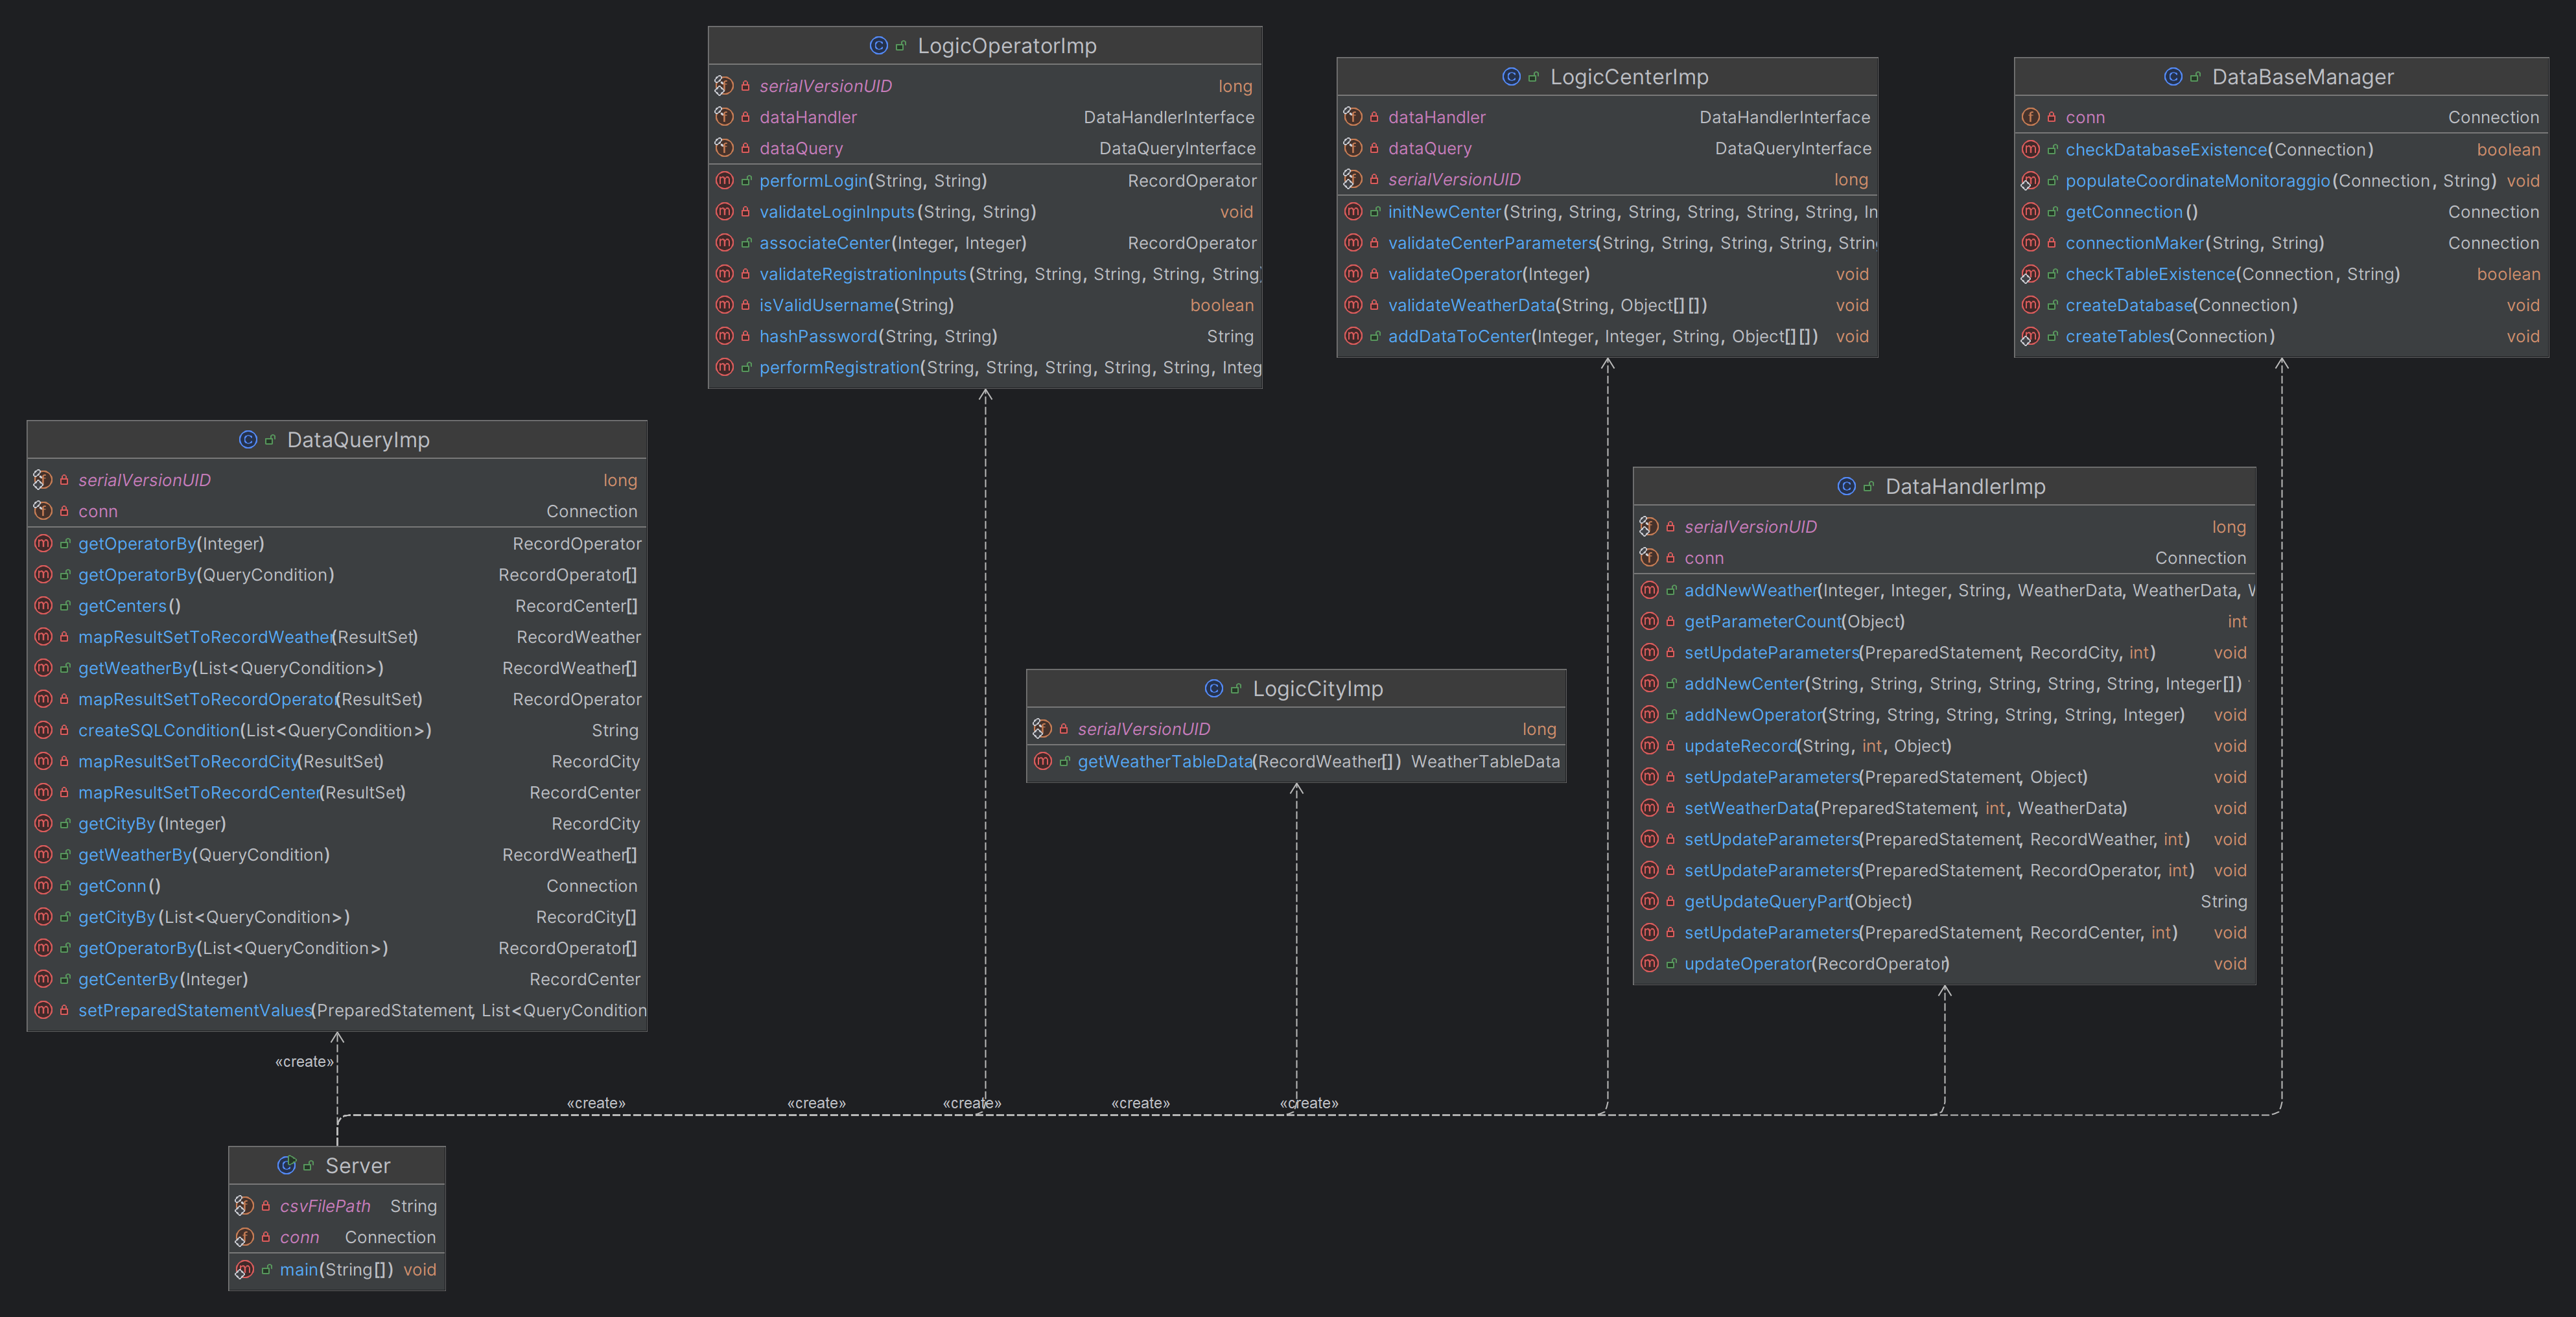
\includegraphics[width=0.9\textwidth]{img/serverPackage.png}
      \caption{UML del package server}
      \label{fig:Server}
\end{figure}

\subsection{Server}
La classe \texttt{Server} è progettata per controllare l'esistenza delle tabelle nel database, se non presenti le crea e popola,
avviare il registro RMI, pubblicare le implementazioni delle interfacce remote.\\
Queste implementazioni sono accessibili ai client remoti, che possoo invocare metodi per interrogare, gestire e manipolare i dati relativi alle operazioni dell'applicazione.\\
In sintesi, \texttt{Server} svolge le seguenti operazioni principali:
\begin{itemize}
      \item \textbf{Creazione connessione al database}: utilizza la classe \texttt{DataBaseManager} per stabilire una connessione al database.
      \item \textbf{Creazione e Configurazione delle Tabelle}: utilizza la classe \texttt{DataBaseManager} per verificare l'esistenza delle tabelle nel database e, se necessario, crearle.
      \item \textbf{Creazione e Configurazione del Registro RMI}: avvia un registro RMI sulla porta specificata (di default, la porta 1099) utilizzando il metodo\\
            \texttt{LocateRegistry.createRegistry(int port)}. Questo registro permette ai client remoti di trovare e invocare i metodi delle interfacce registrate.
      \item \textbf{Inizializzazione delle Implementazioni RMI}: la classe crea istanze delle implementazioni delle interfacce remote che gestiscono diverse logiche di business.
            Queste implementazioni sono
            \begin{itemize}
                  \item \texttt{DataQueryImp}
                  \item \texttt{DataHandlerImp}
                  \item \texttt{LogicOperatorImp}
                  \item \texttt{LogicCenterImp}
                  \item \texttt{LogicCityImp}
            \end{itemize}
      \item \textbf{Registrazione delle Implementazioni nel Registro RMI}: ogni implementazione viene registrata nel registro RMI con un nome specifico utilizzando il metodo
            \texttt{rebind(String name, Remote obj)}. Questo passaggio rende i metodi delle interfacce remote accessibili ai client remoti trmite il nome associato.
\end{itemize}

\subsection{DataBaseManager}
La classe \texttt{DataBaseManager} è progettata per gestire le connessioni al databse e fornire metodi per creare il database, se non esiste, e le relative tabelle.\\
\\
Il costruttore \texttt{public DataBaseManager(String host, String password)} crea una prima connessione al database \texttt{postgres} che, essendo quello creato di defautl,
permette di controllare l'esistenza del database \texttt{climatemonitoring} e di crearlo se non esiste.\\
Poi questa connessione viene chiusa e viene creata una nuova connessione al database \texttt{climatemonitoring} con l'utente \texttt{postgres} e la password fornita.\\
I metodi pubblici sono:
\begin{itemize}
      \item \texttt{public boolean checkDatabaseExistence(Connection conn)}: questo metodo controlla se il database \texttt{climatemonitoring} esiste già.
      \item  \texttt{public static boolean checkTableExistence(Connection conn, String tableName)}: questo metodo controlla se la tabella specificata esiste già nel database.
      \item \texttt{public void createDatabase(Connection conn)}: questo metodo crea il database \texttt{climatemonitoring}.
      \item \texttt{public void createTables(Connection conn)}: questo metodo crea le tabelle \texttt{coordinatemonitoraggio, centrimonitoraggio, operatoriregistrati e parametriclimatici}
      concedendo dei permessi specifici per le tabelle create (vedere capitolo riguardante il Database).
      \item \texttt{public static void populateCoordinateMonitoraggio(Connectionconn, String csvFilePath)}: questo metodo popola la tabella \texttt{coordinatemonitoraggio} con i dati presenti nel file CSV specificato.
      \item \texttt{getConnection()}:
            questo metodo pubblico restituisce l'oggetto \texttt{Connection} gestito da \texttt{ConnectionMaker}. Questo permette ad altre classi del sistema di accedere alla connessione per eseguire operazioni di query, aggiornamento o altre interazioni con il database.
\end{itemize}
I metodi privati sono:
\begin{itemize}
      \item \texttt{connectionMaker(String url, String password)}:
            questo metodo è responsabile della creazione effettiva della connessione al databse. Utilizza l'URL e la password per creare un oggetto \texttt{Connection} tramite il \texttt{DriverManager} di JDBC. Il metodo configura anche un oggetto \texttt{Properties} pre gestire le credenziali di accesso.
\end{itemize}

\subsection{Package implementationRMI}
Il package \texttt{implementationRMI} contiene le classi che implementano le interfacce remote definite nel package \texttt{interfacesRMI} e che gestiscono le logiche di business dell'applicazione.\\

\begin{figure}[H]
      \centering
      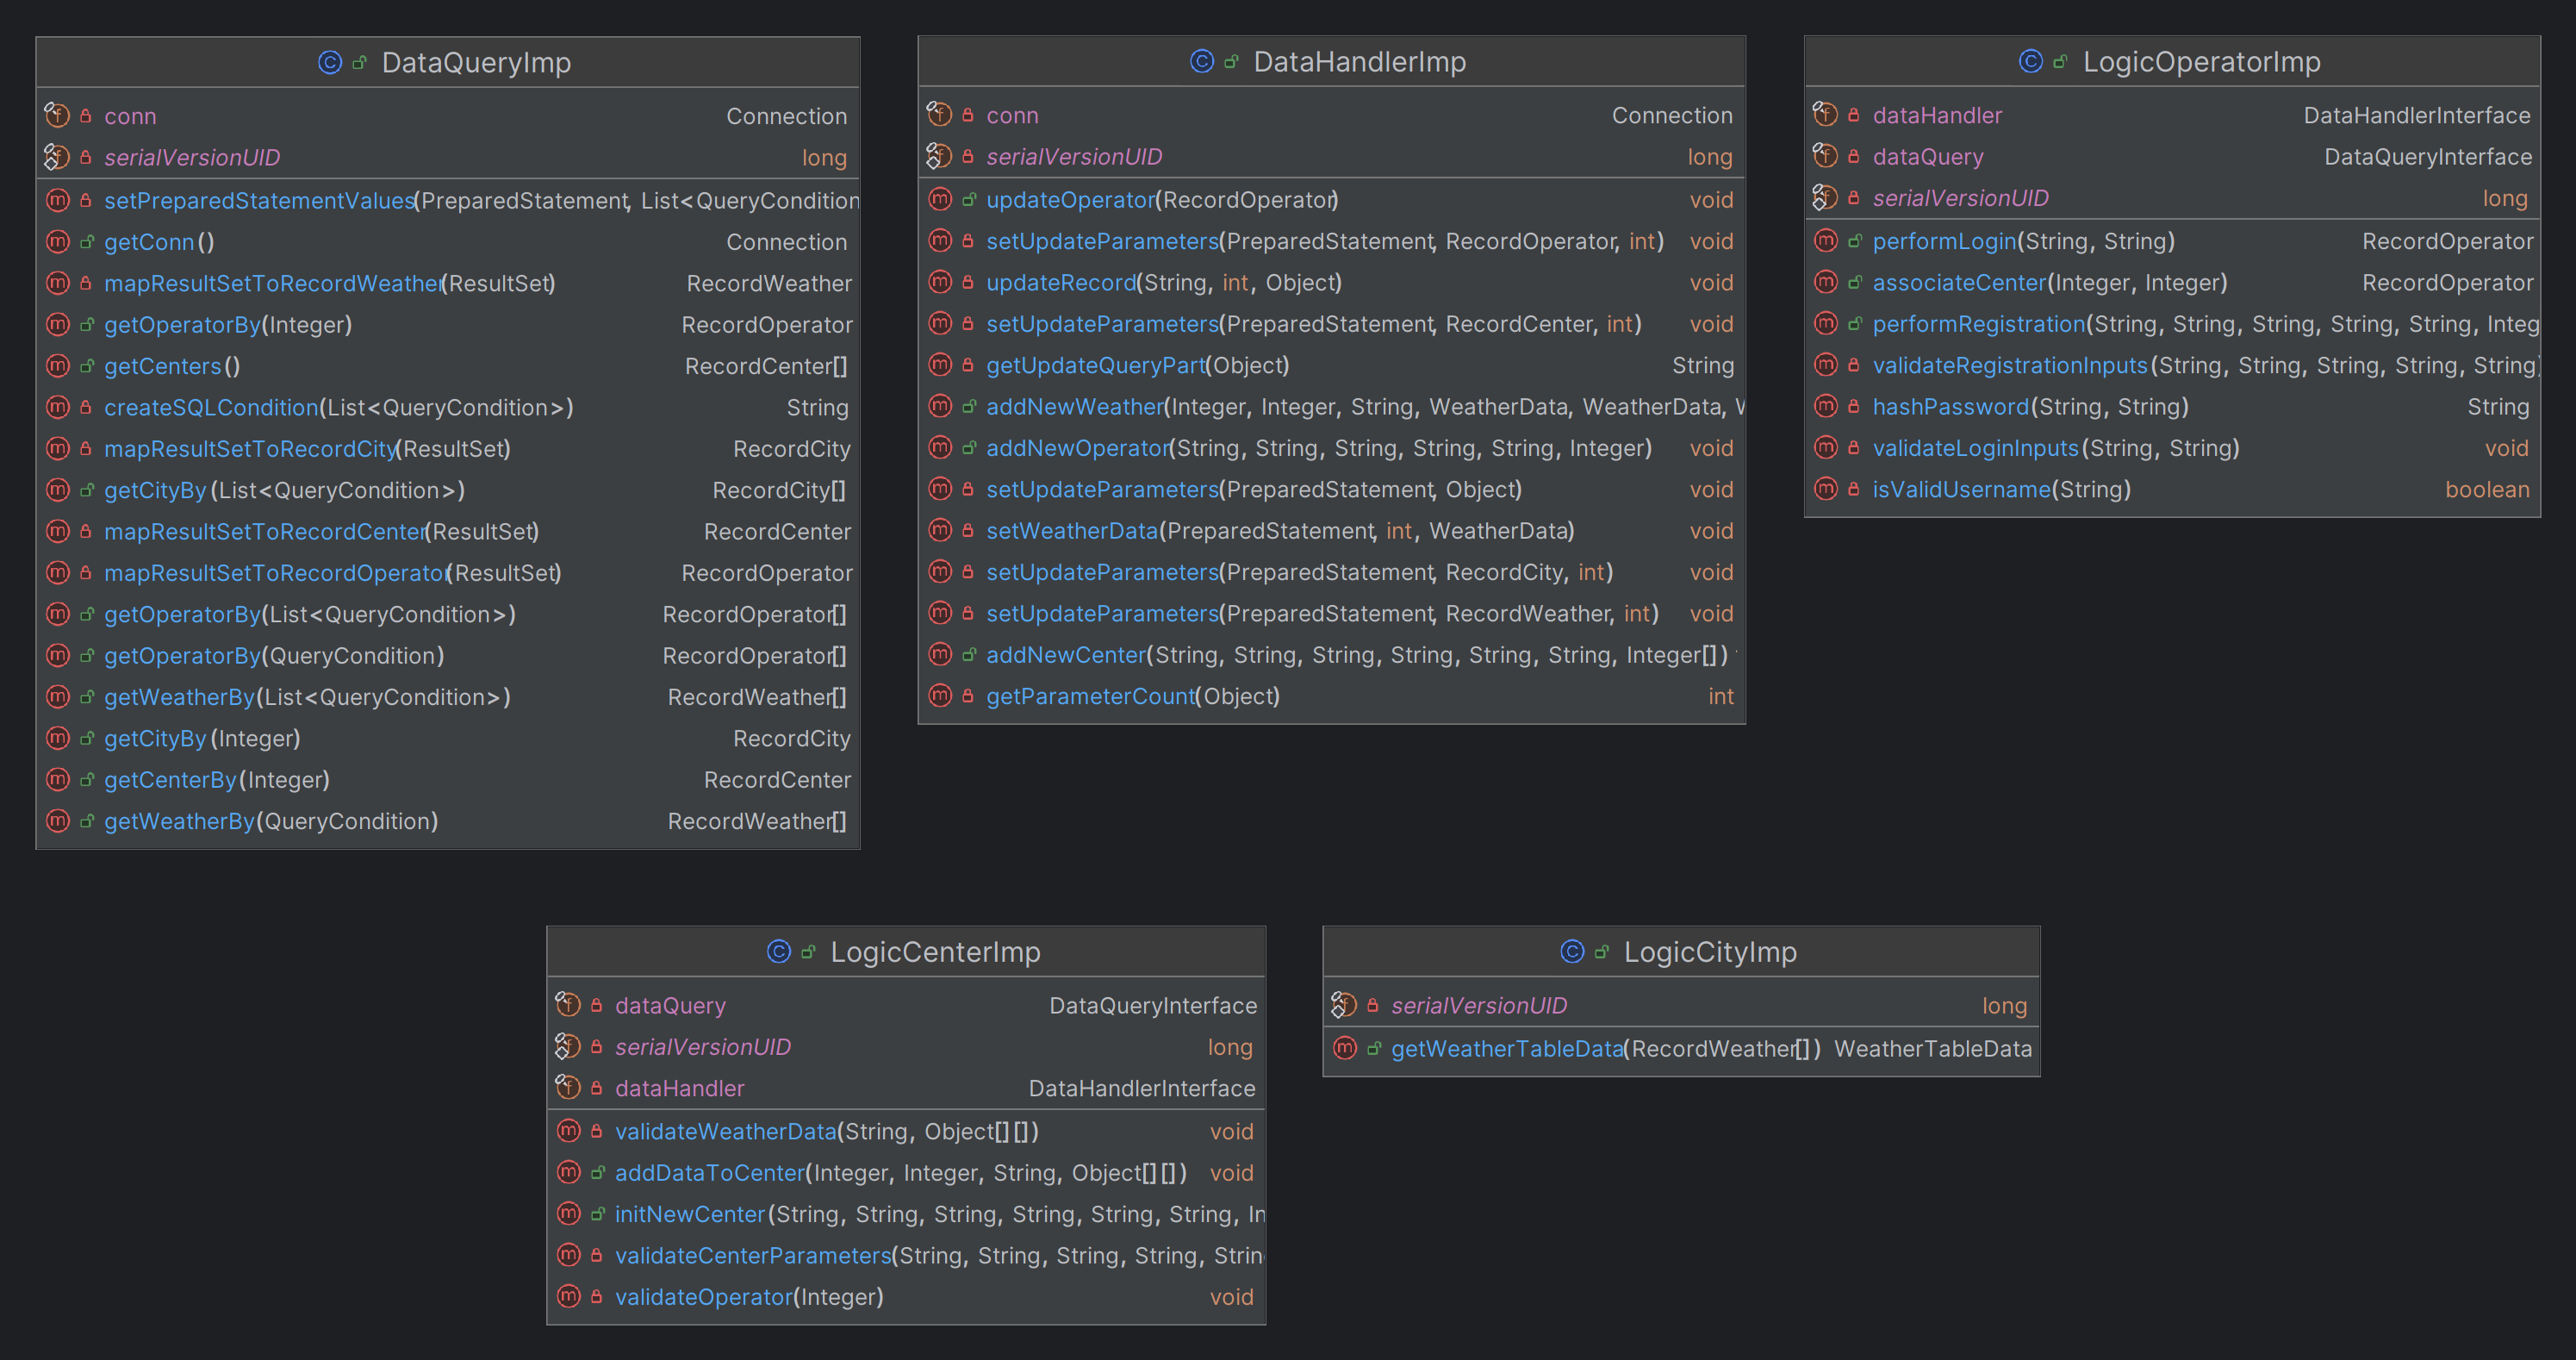
\includegraphics[width=0.9\textwidth]{img/implementatioRMIPackage.png}
      \caption{UML del package implementationRMI}
      \label{fig:implementationRMI}  
\end{figure}

\subsubsection{DataHandlerImp}
La classe \texttt{DataHandlerImp} implementa l'interfaccia \texttt{DataHandlerInterface} e si occupa di gestire operazioni aggiunte e aggiornamento dei record nel database
fornendo un'implementazione dei metodi definiti nell'interfaccia.\\
Questa classe utilizza JDBC per interagire con il database e fornisce metodi per gestire i record relativi agli operatori, ai centri di monitoraggio e ai dati climatici.\\
\\
I metodi pubblici sono:
\begin{itemize}
      \item \texttt{addNewOperator(String nameSurname, String taxcode, String email, String username, String password, Integer centerID)}:
            aggiunge un nuovo operatore al databse. Prima di inserire i dati, viene effettuato un controllo per assicurarsi che l'utente non esista già.
            Lancia eccezioni \texttt{SQLException, RemoteException, IllegalArgumentException} in caso di errori.
      \item \texttt{addNewCenter(String centerName, String streetName, String streetNumber, String CAP, String townName, String districName, Integer[] cityIDs)}:
            aggiunge un nuovo centro di monitoraggio al database. Prima di inserire i dati, viene effettuato un controllo per evitare duplicati. Restituisce un oggetto \texttt{RecordCenter} che rappresenta il centro appena inserito.
            Lancia eccezioni \texttt{SQLException, RemoteException, IllegalArgumentException} in caso di errori.
      \item \texttt{addNewWeather(Integer cityID, Integer centerID, String date, RecordWeather.WeatherData wind, RecordWeather.WeatherData humidity, RecordWeather.WeatherData pressure, RecordWeather.WeatherData temperature, RecordWeather.WeatherData precipitation, RecordWeather.WeatherData glacierElevation, RecordWeather.WeatherData glacierMass)}:
            aggiunge nuovi dati climatici al database associati a una spoecifica città e centro di monitoraggio. Gestisce il formato della data e l'inerimento dei dati climatici in modo dettagliato.
            Lancia eccezioni \texttt{SQLException, RemoteException} in caso di errori.
      \item \texttt{updateOperator(RecordOperator operator)}:
            aggiorna le informazioni di un operatore nel database. Utilizza un metodo interno \texttt{updateRecord} per eseguire l'operazione.
            Lancia eccezioni \texttt{SQLException, RemoteException} in caso di errori.
\end{itemize}
I metodi privati sono:
\begin{itemize}
      \item \texttt{updateRecord(String tableName, int ID, Object record)}:
            esegue l'aggiornamento di un record specifico nel database sulla base del tipo di record e dell'ID fornito.
      \item \texttt{getUpdateQueryPart(Object object)}:
            genera dinamicamente la stringa SQL necessaria per l'aggiornamento di un record di base al tipo di oggetto (ad esempio, \texttt{RecordOperator} o \texttt{RecordCenter}).
      \item \texttt{setUpdateParameters(PreparedStatement stmt, Object object)}:
            imposta i parametri di un oggetto \texttt{PreparedStatement} per l'aggiornamento di un record.
      \item \texttt{setWeatherData(PreparedStatement stmt, int index, RecordWeather.WeatherData data)}:
            imposta i dati climatici (score e commenti) all'interno del \texttt{PreparedStatement} per l'inserimento o l'aggiornamento.
      \item \texttt{getParameterCount(Object record)}:
            restituisce il numero di parametri per un determianto tipo di record, necessario per costruire la query SQL.
\end{itemize}

\subsubsection{DataQueryImp}
La classe \texttt{DataQueryImp} implementa l'interfaccia \texttt{DataQueryInterface} e consente di eseguire query sul database per ottenere informazioni relative a città, operatori, centri di monitoraggioe e dati climatici
fornendo un'implementazione dei metodi definiti nell'interfaccia.\\
\\
I metodi pubblici sono:
\begin{itemize}
      \item \texttt{getCityBy(Integer ID)}: restituisce un oggetto \texttt{RecordCity} contenente le informazioni di una città basandosi sul suo ID.
      \item \texttt{getOperatorBy(Integer ID)}: restituisce un oggetto \texttt{RecordOperator} contenente le informazioni di un operatore basandosi sul suo ID.
      \item \texttt{getCenterBy(Integer ID)}: restituisce un oggetto \texttt{RecordCenter} contenente le informazioni di un centro di monitoraggio basandosi sul suo ID.
      \item \texttt{getCityBy(List<QueryCondition> conditions)}: restituisce un array di oggetti \texttt{RecordCity} contenenti le informazioni di città che soddisfano le condizioni specificate.
      \item \texttt{getOperatorBy(List<QueryCondition> conditions)}: restituisce un array di oggetti \texttt{RecordOperator} contenenti le informazioni di operatori che soddisfano le condizioni specificate.
      \item \texttt{getWeatherBy(List<QueryCondition> conditions)}: restituisce un array di oggetti \texttt{RecordWeather} contenenti le informazioni di dati climatici che soddisfano le condizioni specificate.
      \item \texttt{getCenters()}: restituisce un array di oggetti \texttt{RecordCenter} contenenti le informazioni di tutti i centri di monitoraggio presenti nel database.
      \item \texttt{getConn()}: restituisce l'oggetto \texttt{Connection} utilizzato per la connessione al database.
\end{itemize}
I metodi privati sono:
\begin{itemize}
      \item \texttt{createSQLCondition(List<QueryCondition> conditions)}: crea una stringa SQL di condizione basata su una lista di \texttt{QueryCondition}, usata per costruire dinamicamente le query.
      \item \texttt{setPreparedStatementValues(PreparedStatement stmt, List<QueryCondition> conditions)}: imposta i valori di un oggetto \texttt{PreparedStatement} basandosi su una lista di \texttt{QueryCondition}.
      \item \texttt{mapResultSetToRecordCity(ResultSet rs)}: mappa i risultati di una query SQL su un oggetto \texttt{RecordCity}.
      \item \texttt{mapResultSetToRecordOperator(ResultSet rs)}: mappa i risultati di una query SQL su un oggetto \texttt{RecordOperator}.
      \item \texttt{mapResultSetToRecordCenter(ResultSet rs)}: mappa i risultati di una query SQL su un oggetto \texttt{RecordCenter}.
      \item \texttt{mapResultSetToRecordWeather(ResultSet rs)}: mappa i risultati di una query SQL su un oggetto \texttt{RecordWeather}.
\end{itemize}


\subsubsection{LogicCenterImp}
La classe \texttt{LogicCenterImp} implementa l'interfaccia \texttt{LogicCenterInterface} per la gestione di centri di monitoraggio e dei relativi dati climatici
fornendo un'implementazione dei metodi definiti nell'interfaccia.\\
\\
I metodi pubblici sono:
\begin{itemize}
      \item \texttt{initNewCenter(String centerName, String streetName, String streetNumber, String CAP, String townName, String districtName, Integer[] cityIDs)}:
            questo metodo crea un nuovo centro di monitoraggio con i dati forniti e associa l'operatore corrente al centro appena creato.
            Prima di eseguire queste operazioni, il metodo convalida i parametri utilizzando ilo metodo privato \texttt{validateCenterParameters}.
      \item \texttt{addDataToCenter(Integer centerID, Integer operatorID, String date, Object[][] tableDatas)}:
            questo metodo aggiunge nuovi dati climatici per una città specifica e li associa al centro di monitoraggio gestito dall'operatore indicato.
            Anche in questo caso, i parametri vengono convalidati prima dell'inserimento.
\end{itemize}
I metodi privati sono:
\begin{itemize}
      \item \texttt{validateCenterParameters(String centerName, String streetName, String streetNumber, String CAP, String townName, String districtName, Integer[] cityIDs)}:
            questo metodo privato controlla i parametri forniti per la creazione di un nuovo centro di monitoraggio. Se i parametri non sono validi, viene lanciata un'eccezione.
      \item \texttt{validateOpratorID(Integer operatorID)}:
            questo metodo privato verifica che l'operatore esista e che sia associato a un centro di monitoraggio.
      \item \texttt{validateWeatherData(String date, Object[][] tableDatas)}:
            questo metodo privato verifica che la data fornita sia valida e che almeno uno dei dati climatici non sia nullo.
\end{itemize}

\subsubsection{LogicCityImp}
La classe \texttt{LogicCityImp} implementa l'interfaccia \texttt{LogicCityInterface} per la gestione dei dati climatici associati alle città
fornendo un'implementazione dei metodi definiti nell'interfaccia.\\
\\
E' presente la classe interna statica \texttt{WeatherTableData} che fornisce i metodi per la gestione dei dati climatici.\\
\\
I metodi pubblici sono:
\begin{itemize}
      \item \texttt{public Integer getCategaryAvgScore(String category)}: restituisce la media dei punteggi di una categoria specifica.
      \item \texttt{public int getCategoryRecordCount(String category)}: restituisce il numero di record di una categoria specifica.
      \item \texttt{public List<String> getCategoryComments(String category)}: restituisce una lista di commenti relativi a una categoria specifica.
      \item \texttt{public WheatherTableData getWeatherTableData(RecordWeather[] weatherRecords)}: restituisce un oggetto \texttt{WeatherTableData} che contiene i dati climatici relativi ai record forniti.
\end{itemize}
I metodi privati sono:
\begin{itemize}
      \item \texttt{private void processCatgeory(RecordWeather.WeatherData data, String category)}: questo metodo privato processa i dati climatici di una categoria specifica.
\end{itemize}

\subsubsection{LogicOperatorImp}
La classe \texttt{LogicOperatorImp} implementa l'interfaccia \texttt{LogicOperatorInterface} per la gestione degli operatori e delle operazioni di autenticazione fornendo 
un'implementazione dei metodi definiti nell'interfaccia.\\
Fornisce metodi per la registrazione di nuovi operatori, il login e le verifiche di validità dei dati delgi operatori.\\
\\
I metodi pubblici sono:
\begin{itemize}
      \item \texttt{public RecordOperator performLogin(String username, String password)}: esegue il login di un operatore utilizzando le credenziali fornite.
      \item \texttt{public void performRegistration(String nameSurname, String taxcode, String email, String username, String password, Integer centerID)}: registra un nuovo operatore nel database.
      \item \texttt{public RecordOperator associateCenter(Integer operatorID, Integer centerID)}: modifica i dati dell'operatore per associarlo a un centro di monitoraggio specifico.
\end{itemize}
I metodi privati sono:
\begin{itemize}
      \item \texttt{private boolean isValidUsername(String username)}: verifica che il nome utente fornito sia valido e che non ci sia un duplicato nel database.
      \item \texttt{private String hashPassword(String password)}: genera un hash della password fornita per la memorizzazione sicura nel database.
      \item \texttt{private boolean validateLoginInputs(String username, String password)}: verifica che i dati di login forniti siano validi.
      \item \texttt{private boolean validateRegistrationInputs(String nameSurname, String taxcode, String email, String username, String password)}: verifica che i dati di registrazione forniti siano validi.
\end{itemize}